% =====================================================================================
%  Big Data (ULPGC, 2026-2027) -- Individual Assignment 01
%  Author: Daniel Rodríguez Alonso
%  Build:  cd report && latexmk -pdf main.tex      (or: make report from the folder root)
%  Every number in this file comes from report/generated/*.tex (analysis/make_all.py) or results/.
% =====================================================================================
\documentclass[conference,a4paper]{IEEEtran}
\IEEEoverridecommandlockouts

\usepackage[utf8]{inputenc}
\usepackage[T1]{fontenc}
\usepackage{amsmath,amssymb}
\usepackage{graphicx}
\usepackage{booktabs}
\usepackage{siunitx}
\sisetup{group-separator={\,}, group-minimum-digits=4}
\usepackage[caption=false,font=footnotesize]{subfig}
\usepackage{xcolor}
\usepackage{listings}
\usepackage{microtype}
\usepackage{url}
\usepackage[hidelinks]{hyperref}
\usepackage[capitalise,noabbrev]{cleveref}

\lstset{basicstyle=\ttfamily\footnotesize, columns=fullflexible, breaklines=true,
        frame=single, numbers=none, keepspaces=true}
\graphicspath{{figures/}}

% Key numbers generated by the analysis scripts (\newcommand{\Something}{value})
% Generated by analysis/make_all.py from results/raw/ -- do not edit by hand.
\newcommand{\CFirstIterRelMax}{1.09}
\newcommand{\CFirstIterRelMin}{0.91}
\newcommand{\CflagsChecksumIdentical}{yes}
\newcommand{\CflagsN}{1024}
\newcommand{\CflagsNativeOverOtwo}{0.964}
\newcommand{\CflagsOthreeOverOtwo}{0.957}
\newcommand{\CflagsOtwoMedian}{1.57\,s}
\newcommand{\CflagsOzeroOverOtwo}{2.75}
\newcommand{\ChecksumAllIdentical}{yes}
\newcommand{\ChecksumSizes}{9}
\newcommand{\CorrectMaxAbsErr}{3.55\times 10^{-15}}
\newcommand{\CorrectMaxErrOverBound}{0.141}
\newcommand{\CorrectMaxRelErr}{3.46\times 10^{-12}}
\newcommand{\CorrectNumCases}{9}
\newcommand{\CorrectPassed}{all}
\newcommand{\DenseCommon}{54.0}
\newcommand{\ExpC}{3.45}
\newcommand{\ExpCHi}{3.86}
\newcommand{\ExpCLo}{3.05}
\newcommand{\ExpCNmax}{2048}
\newcommand{\ExpCNmin}{256}
\newcommand{\ExpJava}{3.86}
\newcommand{\ExpJavaHi}{4.27}
\newcommand{\ExpJavaLo}{3.45}
\newcommand{\ExpJavaNmax}{2048}
\newcommand{\ExpJavaNmin}{256}
\newcommand{\ExpLargeC}{3.73}
\newcommand{\ExpLargeCHi}{4.57}
\newcommand{\ExpLargeCLo}{2.90}
\newcommand{\ExpLargeCNmax}{2048}
\newcommand{\ExpLargeCNmin}{512}
\newcommand{\ExpLargeJava}{4.11}
\newcommand{\ExpLargeJavaHi}{5.04}
\newcommand{\ExpLargeJavaLo}{3.19}
\newcommand{\ExpLargeJavaNmax}{2048}
\newcommand{\ExpLargeJavaNmin}{512}
\newcommand{\ExpLargePython}{3.23}
\newcommand{\ExpLargePythonHi}{3.59}
\newcommand{\ExpLargePythonLo}{2.88}
\newcommand{\ExpLargePythonNmax}{1536}
\newcommand{\ExpLargePythonNmin}{512}
\newcommand{\ExpPython}{3.11}
\newcommand{\ExpPythonHi}{3.65}
\newcommand{\ExpPythonLo}{2.58}
\newcommand{\ExpPythonNmax}{1536}
\newcommand{\ExpPythonNmin}{256}
\newcommand{\ExpSmallC}{3.49}
\newcommand{\ExpSmallCHi}{3.67}
\newcommand{\ExpSmallCLo}{3.31}
\newcommand{\ExpSmallCNmax}{512}
\newcommand{\ExpSmallCNmin}{64}
\newcommand{\ExpSmallJava}{3.35}
\newcommand{\ExpSmallJavaHi}{3.61}
\newcommand{\ExpSmallJavaLo}{3.10}
\newcommand{\ExpSmallJavaNmax}{512}
\newcommand{\ExpSmallJavaNmin}{64}
\newcommand{\ExpSmallPython}{3.29}
\newcommand{\ExpSmallPythonHi}{3.91}
\newcommand{\ExpSmallPythonLo}{2.68}
\newcommand{\ExpSmallPythonNmax}{512}
\newcommand{\ExpSmallPythonNmin}{64}
\newcommand{\JavaFirstIterLargeN}{2048}
\newcommand{\JavaFirstIterLargeRel}{1.01}
\newcommand{\JavaFirstIterMaxRel}{6.6}
\newcommand{\JavaFirstIterMaxRelN}{64}
\newcommand{\LoadMax}{8.84}
\newcommand{\LoadMedian}{2.53}
\newcommand{\LoadMin}{0.47}
\newcommand{\MaxAttNC}{2048}
\newcommand{\MaxAttNJava}{2048}
\newcommand{\MaxAttNPython}{2048}
\newcommand{\MaxNC}{2048}
\newcommand{\MaxNJava}{2048}
\newcommand{\MaxNPython}{1536}
\newcommand{\MemCommonN}{1536}
\newcommand{\MemMetricBpeC}{8.0}
\newcommand{\MemMetricBpeJava}{11.5}
\newcommand{\MemMetricBpePython}{32.0}
\newcommand{\MixedPythonFifteenThirtySixSessionThreeK}{2}
\newcommand{\MixedPythonFifteenThirtySixSessionThreeMedian}{281\,s}
\newcommand{\MixedPythonFifteenThirtySixSessionTwoK}{1}
\newcommand{\MixedPythonFifteenThirtySixSessionTwoMedian}{268\,s}
\newcommand{\MixedPythonSevenSixtyEightSessionOneK}{3}
\newcommand{\MixedPythonSevenSixtyEightSessionOneMedian}{34.8\,s}
\newcommand{\MixedPythonSevenSixtyEightSessionTwoK}{2}
\newcommand{\MixedPythonSevenSixtyEightSessionTwoMedian}{30.4\,s}
\newcommand{\NsMaddCFifteenThirtySix}{2.73}
\newcommand{\NsMaddCFiveTwelve}{1.76}
\newcommand{\NsMaddCMax}{4.51}
\newcommand{\NsMaddCMaxN}{2048}
\newcommand{\NsMaddCMin}{0.714}
\newcommand{\NsMaddCMinN}{64}
\newcommand{\NsMaddCOneTwoEight}{0.901}
\newcommand{\NsMaddCSevenSixtyEight}{1.32}
\newcommand{\NsMaddCSixtyFour}{0.714}
\newcommand{\NsMaddCTenTwentyFour}{1.88}
\newcommand{\NsMaddCThreeEightyFour}{1.88}
\newcommand{\NsMaddCTwentyFortyEight}{4.51}
\newcommand{\NsMaddCTwoFiftySix}{1.36}
\newcommand{\NsMaddJavaFifteenThirtySix}{6.78}
\newcommand{\NsMaddJavaFiveTwelve}{2.11}
\newcommand{\NsMaddJavaMax}{7.44}
\newcommand{\NsMaddJavaMaxN}{2048}
\newcommand{\NsMaddJavaMin}{1.02}
\newcommand{\NsMaddJavaMinN}{128}
\newcommand{\NsMaddJavaOneTwoEight}{1.02}
\newcommand{\NsMaddJavaSevenSixtyEight}{1.69}
\newcommand{\NsMaddJavaSixtyFour}{1.06}
\newcommand{\NsMaddJavaTenTwentyFour}{4.16}
\newcommand{\NsMaddJavaThreeEightyFour}{1.77}
\newcommand{\NsMaddJavaTwentyFortyEight}{7.44}
\newcommand{\NsMaddJavaTwoFiftySix}{1.4}
\newcommand{\NsMaddPythonFifteenThirtySix}{77.1}
\newcommand{\NsMaddPythonFiveTwelve}{58.5}
\newcommand{\NsMaddPythonMax}{108}
\newcommand{\NsMaddPythonMaxN}{384}
\newcommand{\NsMaddPythonMin}{42.5}
\newcommand{\NsMaddPythonMinN}{64}
\newcommand{\NsMaddPythonOneTwoEight}{45.7}
\newcommand{\NsMaddPythonSevenSixtyEight}{72.8}
\newcommand{\NsMaddPythonSixtyFour}{42.5}
\newcommand{\NsMaddPythonTenTwentyFour}{72.4}
\newcommand{\NsMaddPythonThreeEightyFour}{108}
\newcommand{\NsMaddPythonTwoFiftySix}{49.4}
\newcommand{\NumMeasuredOk}{128}
\newcommand{\NumRawRows}{364}
\newcommand{\NumSessions}{3}
\newcommand{\NumWarmupRows}{235}
\newcommand{\NumpyVersion}{2.5.4}
\newcommand{\PyExtrapFromN}{1536}
\newcommand{\PyExtrapSeconds}{663}
\newcommand{\PyFailN}{2048}
\newcommand{\PyFailType}{timeout}
\newcommand{\PyFailWall}{600}
\newcommand{\PythonFirstIterRelMax}{1.01}
\newcommand{\PythonFirstIterRelMin}{0.85}
\newcommand{\RatioJavaFifteenThirtySix}{2.48}
\newcommand{\RatioJavaFifteenThirtySixHi}{2.69}
\newcommand{\RatioJavaFifteenThirtySixLo}{2.28}
\newcommand{\RatioJavaFiveTwelve}{1.2}
\newcommand{\RatioJavaFiveTwelveHi}{1.61}
\newcommand{\RatioJavaFiveTwelveLo}{1.01}
\newcommand{\RatioJavaMax}{2.48}
\newcommand{\RatioJavaMaxN}{1536}
\newcommand{\RatioJavaMin}{0.946}
\newcommand{\RatioJavaMinN}{384}
\newcommand{\RatioJavaOneTwoEight}{1.13}
\newcommand{\RatioJavaOneTwoEightHi}{1.22}
\newcommand{\RatioJavaOneTwoEightLo}{0.971}
\newcommand{\RatioJavaSevenSixtyEight}{1.28}
\newcommand{\RatioJavaSevenSixtyEightHi}{1.9}
\newcommand{\RatioJavaSevenSixtyEightLo}{1.08}
\newcommand{\RatioJavaSixtyFour}{1.48}
\newcommand{\RatioJavaSixtyFourHi}{1.73}
\newcommand{\RatioJavaSixtyFourLo}{1.3}
\newcommand{\RatioJavaTenTwentyFour}{2.21}
\newcommand{\RatioJavaTenTwentyFourHi}{3.03}
\newcommand{\RatioJavaTenTwentyFourLo}{1.94}
\newcommand{\RatioJavaThreeEightyFour}{0.946}
\newcommand{\RatioJavaThreeEightyFourHi}{1.2}
\newcommand{\RatioJavaThreeEightyFourLo}{0.738}
\newcommand{\RatioJavaTwentyFortyEight}{1.65}
\newcommand{\RatioJavaTwentyFortyEightHi}{1.7}
\newcommand{\RatioJavaTwentyFortyEightLo}{1.62}
\newcommand{\RatioJavaTwoFiftySix}{1.04}
\newcommand{\RatioJavaTwoFiftySixHi}{1.06}
\newcommand{\RatioJavaTwoFiftySixLo}{0.926}
\newcommand{\RatioPythonFifteenThirtySix}{28.2}
\newcommand{\RatioPythonFifteenThirtySixHi}{30.5}
\newcommand{\RatioPythonFifteenThirtySixLo}{25.9}
\newcommand{\RatioPythonFiveTwelve}{33.2}
\newcommand{\RatioPythonFiveTwelveHi}{38.7}
\newcommand{\RatioPythonFiveTwelveLo}{29.2}
\newcommand{\RatioPythonMax}{59.5}
\newcommand{\RatioPythonMaxN}{64}
\newcommand{\RatioPythonMin}{28.2}
\newcommand{\RatioPythonMinN}{1536}
\newcommand{\RatioPythonOneTwoEight}{50.7}
\newcommand{\RatioPythonOneTwoEightHi}{51.9}
\newcommand{\RatioPythonOneTwoEightLo}{43.1}
\newcommand{\RatioPythonSevenSixtyEight}{55.2}
\newcommand{\RatioPythonSevenSixtyEightHi}{61.2}
\newcommand{\RatioPythonSevenSixtyEightLo}{49.5}
\newcommand{\RatioPythonSixtyFour}{59.5}
\newcommand{\RatioPythonSixtyFourHi}{62.2}
\newcommand{\RatioPythonSixtyFourLo}{52.1}
\newcommand{\RatioPythonTenTwentyFour}{38.4}
\newcommand{\RatioPythonTenTwentyFourHi}{47.5}
\newcommand{\RatioPythonTenTwentyFourLo}{34.7}
\newcommand{\RatioPythonThreeEightyFour}{57.4}
\newcommand{\RatioPythonThreeEightyFourHi}{63.8}
\newcommand{\RatioPythonThreeEightyFourLo}{37.9}
\newcommand{\RatioPythonTwoFiftySix}{36.4}
\newcommand{\RatioPythonTwoFiftySixHi}{44.6}
\newcommand{\RatioPythonTwoFiftySixLo}{32.2}
\newcommand{\RelIQRCMax}{23.0}
\newcommand{\RelIQRCMaxN}{384}
\newcommand{\RelIQRCMedian}{4.1}
\newcommand{\RelIQRJavaMax}{21.7}
\newcommand{\RelIQRJavaMaxN}{384}
\newcommand{\RelIQRJavaMedian}{5.9}
\newcommand{\RelIQRPythonMax}{18.4}
\newcommand{\RelIQRPythonMaxN}{384}
\newcommand{\RelIQRPythonMedian}{10.8}
\newcommand{\RssBaseC}{1.9}
\newcommand{\RssBaseJava}{48.2}
\newcommand{\RssBasePython}{12.5}
\newcommand{\RssCFifteenThirtySix}{55.8}
\newcommand{\RssCFiveTwelve}{8.0}
\newcommand{\RssCOneTwoEight}{2.3}
\newcommand{\RssCSevenSixtyEight}{15.5}
\newcommand{\RssCSixtyFour}{2.0}
\newcommand{\RssCTenTwentyFour}{25.8}
\newcommand{\RssCThreeEightyFour}{5.3}
\newcommand{\RssCTwentyFortyEight}{97.9}
\newcommand{\RssCTwoFiftySix}{3.4}
\newcommand{\RssCommonC}{55.8}
\newcommand{\RssCommonJava}{142.4}
\newcommand{\RssCommonPython}{283.4}
\newcommand{\RssJavaFifteenThirtySix}{142.4}
\newcommand{\RssJavaFiveTwelve}{54.9}
\newcommand{\RssJavaOneTwoEight}{49.4}
\newcommand{\RssJavaSevenSixtyEight}{62.7}
\newcommand{\RssJavaSixtyFour}{49.3}
\newcommand{\RssJavaTenTwentyFour}{72.4}
\newcommand{\RssJavaThreeEightyFour}{52.5}
\newcommand{\RssJavaTwentyFortyEight}{184.7}
\newcommand{\RssJavaTwoFiftySix}{50.7}
\newcommand{\RssMaxNC}{97.9}
\newcommand{\RssMaxNJava}{184.7}
\newcommand{\RssMaxNPython}{283.4}
\newcommand{\RssMaxNnC}{2048}
\newcommand{\RssMaxNnJava}{2048}
\newcommand{\RssMaxNnPython}{1536}
\newcommand{\RssNetCommonC}{54.0}
\newcommand{\RssNetCommonJava}{94.2}
\newcommand{\RssNetCommonPython}{270.9}
\newcommand{\RssOverDenseC}{1.00}
\newcommand{\RssOverDenseJava}{1.42}
\newcommand{\RssOverDensePython}{5.02}
\newcommand{\RssPythonFifteenThirtySix}{283.4}
\newcommand{\RssPythonFiveTwelve}{42.5}
\newcommand{\RssPythonOneTwoEight}{14.4}
\newcommand{\RssPythonSevenSixtyEight}{79.9}
\newcommand{\RssPythonSixtyFour}{12.8}
\newcommand{\RssPythonTenTwentyFour}{132.9}
\newcommand{\RssPythonThreeEightyFour}{29.4}
\newcommand{\RssPythonTwoFiftySix}{19.9}
\newcommand{\SessionOneEnd}{23:01}
\newcommand{\SessionOneLoadMax}{8.84}
\newcommand{\SessionOneLoadMedian}{2.64}
\newcommand{\SessionOneStart}{2026-10-27 22:48}
\newcommand{\SessionThreeEnd}{17:34}
\newcommand{\SessionThreeLoadMax}{1.50}
\newcommand{\SessionThreeLoadMedian}{1.06}
\newcommand{\SessionThreeStart}{2026-10-29 16:57}
\newcommand{\SessionTwoEnd}{11:00}
\newcommand{\SessionTwoLoadMax}{1.51}
\newcommand{\SessionTwoLoadMedian}{1.19}
\newcommand{\SessionTwoStart}{2026-10-29 10:46}
\newcommand{\SweepEnd}{17:34}
\newcommand{\SweepMachineMinutes}{57}
\newcommand{\SweepStart}{2026-10-27 22:48}
\newcommand{\TCFifteenThirtySix}{9.9\,s}
\newcommand{\TCFifteenThirtySixIQR}{457\,ms}
\newcommand{\TCFifteenThirtySixK}{5}
\newcommand{\TCFiveTwelve}{237\,ms}
\newcommand{\TCFiveTwelveIQR}{8.74\,ms}
\newcommand{\TCFiveTwelveK}{5}
\newcommand{\TCOneTwoEight}{1.89\,ms}
\newcommand{\TCOneTwoEightIQR}{76.1\,\textmu s}
\newcommand{\TCOneTwoEightK}{5}
\newcommand{\TCSevenSixtyEight}{597\,ms}
\newcommand{\TCSevenSixtyEightIQR}{27.8\,ms}
\newcommand{\TCSevenSixtyEightK}{5}
\newcommand{\TCSixtyFour}{187\,\textmu s}
\newcommand{\TCSixtyFourIQR}{7.59\,\textmu s}
\newcommand{\TCSixtyFourK}{5}
\newcommand{\TCTenTwentyFour}{2.02\,s}
\newcommand{\TCTenTwentyFourIQR}{283\,ms}
\newcommand{\TCTenTwentyFourK}{5}
\newcommand{\TCThreeEightyFour}{106\,ms}
\newcommand{\TCThreeEightyFourIQR}{24.5\,ms}
\newcommand{\TCThreeEightyFourK}{5}
\newcommand{\TCTwentyFortyEight}{38.8\,s}
\newcommand{\TCTwentyFortyEightIQR}{592\,ms}
\newcommand{\TCTwentyFortyEightK}{5}
\newcommand{\TCTwoFiftySix}{22.8\,ms}
\newcommand{\TCTwoFiftySixIQR}{226\,\textmu s}
\newcommand{\TCTwoFiftySixK}{5}
\newcommand{\TJavaFifteenThirtySix}{24.6\,s}
\newcommand{\TJavaFifteenThirtySixIQR}{163\,ms}
\newcommand{\TJavaFifteenThirtySixK}{5}
\newcommand{\TJavaFiveTwelve}{284\,ms}
\newcommand{\TJavaFiveTwelveIQR}{36.5\,ms}
\newcommand{\TJavaFiveTwelveK}{5}
\newcommand{\TJavaOneTwoEight}{2.13\,ms}
\newcommand{\TJavaOneTwoEightIQR}{89.4\,\textmu s}
\newcommand{\TJavaOneTwoEightK}{5}
\newcommand{\TJavaSevenSixtyEight}{764\,ms}
\newcommand{\TJavaSevenSixtyEightIQR}{127\,ms}
\newcommand{\TJavaSevenSixtyEightK}{5}
\newcommand{\TJavaSixtyFour}{278\,\textmu s}
\newcommand{\TJavaSixtyFourIQR}{16.5\,\textmu s}
\newcommand{\TJavaSixtyFourK}{5}
\newcommand{\TJavaTenTwentyFour}{4.47\,s}
\newcommand{\TJavaTenTwentyFourIQR}{415\,ms}
\newcommand{\TJavaTenTwentyFourK}{5}
\newcommand{\TJavaThreeEightyFour}{100\,ms}
\newcommand{\TJavaThreeEightyFourIQR}{21.8\,ms}
\newcommand{\TJavaThreeEightyFourK}{5}
\newcommand{\TJavaTwentyFortyEight}{64\,s}
\newcommand{\TJavaTwentyFortyEightIQR}{1.62\,s}
\newcommand{\TJavaTwentyFortyEightK}{5}
\newcommand{\TJavaTwoFiftySix}{23.6\,ms}
\newcommand{\TJavaTwoFiftySixIQR}{666\,\textmu s}
\newcommand{\TJavaTwoFiftySixK}{5}
\newcommand{\TPythonFifteenThirtySix}{280\,s}
\newcommand{\TPythonFifteenThirtySixIQR}{7\,s}
\newcommand{\TPythonFifteenThirtySixK}{3}
\newcommand{\TPythonFiveTwelve}{7.85\,s}
\newcommand{\TPythonFiveTwelveIQR}{955\,ms}
\newcommand{\TPythonFiveTwelveK}{5}
\newcommand{\TPythonOneTwoEight}{95.8\,ms}
\newcommand{\TPythonOneTwoEightIQR}{10.5\,ms}
\newcommand{\TPythonOneTwoEightK}{5}
\newcommand{\TPythonSevenSixtyEight}{33\,s}
\newcommand{\TPythonSevenSixtyEightIQR}{4.36\,s}
\newcommand{\TPythonSevenSixtyEightK}{5}
\newcommand{\TPythonSixtyFour}{11.1\,ms}
\newcommand{\TPythonSixtyFourIQR}{136\,\textmu s}
\newcommand{\TPythonSixtyFourK}{5}
\newcommand{\TPythonTenTwentyFour}{77.8\,s}
\newcommand{\TPythonTenTwentyFourIQR}{3.13\,s}
\newcommand{\TPythonTenTwentyFourK}{5}
\newcommand{\TPythonThreeEightyFour}{6.1\,s}
\newcommand{\TPythonThreeEightyFourIQR}{1.12\,s}
\newcommand{\TPythonThreeEightyFourK}{5}
\newcommand{\TPythonTwoFiftySix}{828\,ms}
\newcommand{\TPythonTwoFiftySixIQR}{88.5\,ms}
\newcommand{\TPythonTwoFiftySixK}{5}


\begin{document}

\title{Runtime and Memory Scaling of Naive Dense Matrix Multiplication in Python, Java and C\\[0.3em]
\large Big Data -- Individual Assignment 01}

\author{\IEEEauthorblockN{Daniel Rodríguez Alonso}
\IEEEauthorblockA{Grado en Ciencia e Ingeniería de Datos\\
Universidad de Las Palmas de Gran Canaria (ULPGC)\\
Big Data, Academic Year 2026--2027}}

\maketitle

% ------------------------------------------------------------------ Abstract
\begin{abstract}
This study compares the runtime and memory of the same naive triple-loop (ijk) float64 matrix multiplication
implemented in C (gcc -O2), Java (OpenJDK~21) and Python (CPython~3.12) on one Intel Core i7-9750H laptop, for
square matrices with $n$ from 64 to 2048. The three programs read shared input files and produce bit-identical
results. Only the kernel is timed, with five separate process runs per configuration (three for Python at $n=1536$), summarised by the median and
the interquartile range. C and Java completed all sizes. Python completed $n=1536$ (median
\TPythonFifteenThirtySix) and exceeded the 600\,s limit at $n=2048$. The fitted growth exponent is
\ExpPython{} [95\,\% CI \ExpPythonLo, \ExpPythonHi] for Python but \ExpC{} [\ExpCLo, \ExpCHi] for C and
\ExpJava{} [\ExpJavaLo, \ExpJavaHi] for Java, because their time per multiply--add rises with $n$ (C: from
\NsMaddCMin{} to \NsMaddCMax\,ns). Java is indistinguishable from C for $128\le n\le384$ and up to
\RatioJavaMax{} times slower for larger $n$; Python is \RatioPythonMin--\RatioPythonMax{} times slower than C. At
$n=\MemCommonN$ the peak resident memory above the runtime baseline is \RssNetCommonPython{}\,MiB for Python
against \RssNetCommonC{}\,MiB for C. The conclusions are limited to this machine, these toolchains and these
settings.
\end{abstract}

\begin{IEEEkeywords}
matrix multiplication, benchmarking, performance evaluation, programming languages, JIT compilation,
memory hierarchy, peak resident set size
\end{IEEEkeywords}

% ------------------------------------------------------------------ Introduction
\section{Introduction and Objective}
\label{sec:intro}
Dense matrix multiplication is a building block of many data-intensive workloads (linear models, similarity
computations, neural-network layers). Its classical definition needs $n^3$ multiply--add operations for two
$n\times n$ matrices, so the cost of an implementation grows quickly with the data size, and the constant factor
in front of $n^3$ is decided by the language runtime, the data layout and the memory hierarchy. This report is the
first of four related studies; it establishes a validated sequential baseline that the later assignments
(optimisation, sparse matrices, parallel and distributed execution) reuse.

\textbf{Research question (RQ).} \emph{On one Intel Core i7-9750H laptop, how do the runtime and the memory use of
the same naive triple-loop float64 matrix multiplication grow with the matrix size $n$ when it is implemented in C,
Java and Python, and how large are the differences between the three implementations at equal $n$?}
The factor varied is $n$ (side length of square $n\times n$ matrices) for each of three implementations; the
outcomes are the kernel runtime, the time per multiply--add, the peak memory of the process and the largest
feasible $n$ under fixed budgets.

\textbf{Hypotheses (predictions stated before the measurements).}
\emph{H1:} the runtime of every implementation grows approximately as $n^3$ (fitted exponent $b\approx3$), with
possible deviations at large $n$ when the working set leaves the caches.
\emph{H2:} at equal $n$ the order is C $<$ Java $<$ Python; after just-in-time (JIT) warm-up Java is within a small
factor of C, while Python is one to two orders of magnitude slower.
\emph{H3:} Python needs several times more memory per matrix element than C and Java, because every element is a
boxed object.

The study contributes (i) three implementations with identical loop order that produce bit-identical results,
(ii) a protocol with shared input files, a common timing boundary and recorded failures, and (iii) runtime,
growth-exponent and memory measurements with their variability.

% ------------------------------------------------------------------ Background
\section{Background and Related Work}
\label{sec:background}
\textbf{Classical algorithm.} For $C=AB$, $c_{ij}=\sum_{k=0}^{n-1} a_{ik}b_{kj}$, which costs $n^3$ multiplications
and $n^3$ additions ($2n^3$ floating-point operations); the three nested loops can be written in six orders that
perform the same arithmetic but access memory differently~\cite{golub2013}. In the ijk order with row-major storage
used here, the innermost loop reads a row of $A$ with unit stride and a column of $B$ with stride $n$, i.e.\ every
access to $B$ touches a different cache line. Once $B$ ($8n^2$ bytes) no longer fits in a cache level, the
column walk causes cache and translation-lookaside-buffer (TLB) misses; Drepper uses exactly this matrix
multiplication to illustrate the effect of access patterns on the memory hierarchy~\cite{drepper2007}, and Lam
et al.\ show that cache interference in matrix kernels depends strongly on the access stride and the matrix
size~\cite{lam1991}. High-performance libraries avoid these costs with blocking and packing~\cite{goto2008}; such
optimisations are deliberately excluded here and are the subject of Assignment~2.

\textbf{Language runtimes.} C is compiled ahead of time to machine code. Java bytecode is first interpreted and then
compiled at run time by the HotSpot JIT compiler, so early iterations are slower and timings vary between
virtual-machine invocations; Georges et al.\ recommend steady-state measurements and several VM invocations for
this reason~\cite{georges2007}. Since JDK~17 all Java floating-point operations are strict~\cite{jep306}.
CPython~3.12 executes bytecode in an interpreter that specialises instructions adaptively at run time but does not
generate machine code~\cite{pep659}; each Python \texttt{float} is a separate heap object, and a \texttt{list} stores
references to such objects. \texttt{sys.getsizeof} reports only the memory directly attributed to an object, not to
the objects it refers to~\cite{pydocsys}.

\textbf{Numerical accuracy.} A dot product of length $n$ computed in floating point satisfies
$|\hat{c}_{ij}-c_{ij}|\le\gamma_n(|A||B|)_{ij}$ with $\gamma_n=nu/(1-nu)$ and unit round-off $u=2^{-53}$ for
float64~\cite{higham2002}. Different summation orders therefore give slightly different results, while the same
order and the same IEEE~754 operations give identical results.

\textbf{Benchmarking methodology.} Hoefler and Belli recommend reporting medians and non-parametric variability
measures, the number of repetitions and the full experimental setup~\cite{hoefler2015}; Mytkowicz et al.\ show that
seemingly innocuous aspects of the setup can bias conclusions~\cite{mytkowicz2009}, which motivates scoping the
conclusions to the tested environment.

% ------------------------------------------------------------------ Methodology
\section{Methodology}
\label{sec:method}

\subsection{Implementations}
The three programs (\texttt{src/c}, \texttt{src/java}, \texttt{src/python}) implement the same kernel:
\begin{lstlisting}
for i in 0..n-1:
  for j in 0..n-1:
    s = 0.0
    for k in 0..n-1: s += A[i][k] * B[k][j]
    C[i][j] = s
\end{lstlisting}
with float64 values (\texttt{double} in C and Java, \texttt{float} in Python), the same ijk order and a scalar
accumulator, so the floating-point evaluation order is identical. Each language uses its idiomatic storage, which
is the main unavoidable difference: \emph{C} stores each matrix in one contiguous row-major block
(\texttt{malloc}/\texttt{calloc}, element $(i,j)$ at \texttt{M[i*n+j]}); \emph{Java} uses \texttt{double[][]}, an
array of separately allocated row arrays, so \texttt{b[k][j]} first loads the reference to row $k$ and then the
element, with bounds checks managed by the JIT; \emph{Python} uses a list of row lists of \texttt{float} objects, so
every access dereferences a pointer to a boxed value and every multiply--add is executed by the interpreter and
allocates a new \texttt{float}. Java and Python hoist the row references \texttt{A[i]} and \texttt{C[i]} out of
the inner loops; C computes the flat index. No library routine is used in any kernel; NumPy~\cite{harris2020} is
used only to generate the inputs and as the reference in the correctness tests.

\textbf{Fixed settings.} C: gcc~13.3.0 with \texttt{-O2 -std=c11 -Wall -Wextra}, default x86-64 target (SSE2, no
\texttt{-march}), no \texttt{-ffast-math}, single thread; the generated assembly of the kernel contains only scalar
\texttt{mulsd}/\texttt{addsd} instructions (no vectorisation and no fused multiply--add, FMA). Java: OpenJDK
21.0.12.1, \texttt{javac --release 21}, \texttt{java -Xms1g -Xmx4g -XX:+UseG1GC}, default tiered JIT. Python:
CPython~3.12.3, standard library only. The kernel runs on one thread in every language (the JVM keeps its
background JIT and garbage-collection threads); \texttt{OMP\_NUM\_THREADS}, \texttt{OPENBLAS\_NUM\_THREADS} and
\texttt{MKL\_NUM\_THREADS} are set to~1 for every run.

\subsection{Inputs}
All programs read the same files, generated once by \texttt{scripts/gen\_inputs.py}: NumPy
\texttt{default\_rng(42)} (PCG64), $A$ drawn first and then $B$, independent uniform values in $[-1,1)$, stored as
raw little-endian float64 in row-major order with a JSON sidecar and SHA-256 checksums. Since $|c_{ij}|\le n$, no
overflow can occur. Loading the files, building the language-specific structure and allocating $C$ happen before
the timed region.

\subsection{Experimental environment}
\begin{table}[t]
\centering
\caption{Execution environment (\texttt{results/environment.md}, captured by \texttt{capture\_env.sh}).}
\label{tab:env}
\footnotesize
\begin{tabular}{@{}lp{0.70\columnwidth}@{}}
\toprule
Item & Value \\
\midrule
CPU & Intel Core i7-9750H, 1 socket, 6 cores / 12 threads, 2.6\,GHz base, 4.5\,GHz max, AVX2/FMA \\
Caches & L1d 32\,KiB and L2 256\,KiB per core; L3 12\,MiB shared \\
Frequency & governor \texttt{powersave}, turbo enabled, AC power connected \\
Memory & 15\,GiB (16.6\,GB) RAM \\
OS & Ubuntu 24.04.5 LTS, Linux 7.0.0-38-generic, x86-64 \\
C & gcc 13.3.0, \texttt{-O2 -std=c11 -Wall -Wextra} \\
Java & OpenJDK 21.0.12.1 (HotSpot 64-bit Server VM), \texttt{-Xms1g -Xmx4g -XX:+UseG1GC} \\
Python & CPython 3.12.3 (venv) \\
Tools & NumPy \NumpyVersion{} (inputs, reference), GNU \texttt{time} (RSS) \\
Threads & kernel single-threaded; \texttt{OMP/OPENBLAS/MKL\_NUM\_THREADS=1} \\
\bottomrule
\end{tabular}
\end{table}
\Cref{tab:env} summarises the machine. The laptop was shared with three other benchmark sessions of related
assignments; all timed runs were serialised by a machine-wide file lock (\cref{sec:protocol}).

\subsection{Correctness validation}
Before any benchmark, \texttt{tests/test\_correctness.py} runs the three benchmarked programs as black boxes and
checks (\cref{tab:correctness}): known products with exact answers ($1\times1$, $2\times2$ and a non-symmetric
$3\times3$ with small integers), $AI=A$, $IB=B$ and $A\cdot0=0$ for $n=7$ (exact), and random uniform inputs for
$n\in\{7,64,100\}$ against NumPy with the element-wise tolerance $|c_{ij}-c^{\mathrm{ref}}_{ij}|\le 2nu(|A||B|)_{ij}$.
The factor 2 accounts for both results carrying an error of at most $\gamma_n(|A||B|)_{ij}\approx nu(|A||B|)_{ij}$,
since NumPy sums in a different order. Results of the three own implementations must be bit-identical, because they
perform the same IEEE~754 operations in the same order. During the benchmark the checksum $\sum_{ij}c_{ij}$ printed
after every repetition is compared across languages at every $n$.

\subsection{Measurement protocol and budgets}
\label{sec:protocol}
\textbf{Timer and boundary.} Each program measures the kernel only (boundary \emph{kernel}) with a monotonic clock:
\texttt{clock\_gettime(CLOCK\_MONOTONIC)} in C, \texttt{System.nanoTime()} in Java and
\texttt{time.perf\_counter\_ns()} in Python. Input loading, allocation and zeroing of $C$ and the checksum are
excluded. Printing the checksum consumes the result, which prevents dead-code elimination. For short kernels a
sample times a batch of $\lceil 0.2\,\mathrm{s}/t_{\mathrm{w}}\rceil$ consecutive calls ($t_{\mathrm{w}}$: last
warm-up time) and reports the time per multiplication; the batch size is stored with every row.

\textbf{Repetitions and warm-up.} A configuration (language, $n$) consists of $P$ separate process runs; each
process performs $W$ in-process warm-up repetitions (recorded, excluded from statistics) and one measured
repetition, giving $k=P$ samples that include between-process variability~\cite{georges2007}. A pilot
(\texttt{results/raw/pilot\_size\_sweep.csv}) showed a strong JIT effect in Java and no warm-up effect in C at
$n=1024$ or in Python at $n=512$. Within the 90-minute budget this led to: C $W=2$ ($n\le512$), 1 ($n=768$), 0
($n\ge1024$); Java $W=5$ ($n\le512$), 2 ($n\le1024$), 1 ($n\ge1536$); Python $W=1$ ($n\le512$), 0 ($n\ge768$);
$P=5$ everywhere except Python at $n=1536$ ($P=3$, about six minutes per run) and $n=2048$ (one attempt to
document the time limit). The order of the languages was shuffled at every $n$ (fixed seed).

\textbf{Memory.} The common metric is the \emph{peak resident set size} (RSS) of the whole process, measured by
GNU \texttt{time} (\texttt{\%M})~\cite{gnutime} for every process run; it includes the interpreter or virtual
machine. To separate this runtime baseline, the same programs were run at $n=1$ ($k=5$). Each program also reports
one language-internal metric, which is not comparable across languages: C \texttt{matrix\_storage\_bytes} (the exact
$3\cdot8n^2$ bytes allocated), Java \texttt{jvm\_heap\_peak\_used\_bytes} (sum of the peak usage of the heap
\texttt{MemoryPoolMXBean}s~\cite{javampool}) and Python \texttt{pyobj\_deep\_size\_bytes} (\texttt{sys.getsizeof}
of the outer lists, row lists and every element, measured outside the timed region).

\textbf{Sizes, budgets and stopping rule.} Declared sequence $n\in\{64,128,256,384,512,768,1024,1536,2048\}$,
mixing powers of two with $384=3\cdot2^7$, $768$ and $1536$. Budgets fixed before the large runs: 600\,s per
process run, 8\,GB of memory, at most 90\,minutes of benchmark time for the whole study. Dense storage needs
$3\cdot8n^2$ bytes (96\,MiB at $n=2048$), so memory is not the limiting resource. A run that exceeds a limit is
recorded with its status and an empty time, and larger sizes of that language are not attempted.

\textbf{Execution and statistics.} Every configuration ran through \texttt{run\_measured.py}, which holds a
machine-wide lock while measuring, records the process wall time, peak RSS, exit status and the 1-minute load
average, and appends one raw CSV row per repetition. The sweep was interrupted and resumed, so it ran in
\NumSessions{} measurement sessions (a new session starts after a gap of more than one hour between rows):
session~1, \SessionOneStart{}--\SessionOneEnd{}, all languages for $n\le512$ plus C, Java and three Python runs at
$n=768$ (median load average \SessionOneLoadMedian{}, maximum \SessionOneLoadMax{}, with a browser and other
assignments active); session~2, \SessionTwoStart{}--\SessionTwoEnd{} after a fresh boot, the remaining two Python
runs at $n=768$, all languages at $n=1024$ and the first Python run at $n=1536$ (median load
\SessionTwoLoadMedian{}); session~3, \SessionThreeStart{}--\SessionThreeEnd{}, the rest of $n=1536$, $n=2048$ and
the C flags study (median load \SessionThreeLoadMedian{}). In total the sweep produced \NumRawRows{} raw rows
(\NumWarmupRows{} of them warm-ups) and used about \SweepMachineMinutes{} minutes of process time. For each
configuration the report gives the median and
the interquartile range (IQR $=Q_3-Q_1$) of the $k$ measured samples. No measurement was excluded. The growth
exponent $b$ in $T\approx c\,n^b$ is fitted by least squares on $\log T$ vs.\ $\log n$ of the medians, with a 95\,\%
confidence interval from the Student $t$ distribution; runtime ratios at equal $n$ use the ratio of medians with a
95\,\% bootstrap interval (5000 resamples).

\textbf{Separate experiment: C compiler flags.} Outside the controlled comparison, the same C source was compiled
with \texttt{-O0}, \texttt{-O2}, \texttt{-O3} and \texttt{-O3 -march=native} (all with \texttt{-std=c11})~\cite{gccopt}
and run at $n\in\{256,512,1024\}$ with $P=5$ process runs of $W=1$ warm-up and one measured repetition each
(\texttt{results/raw/c\_flags.csv}).

% ------------------------------------------------------------------ Results
\section{Results}
\label{sec:results}

\begin{table}[t]
\centering
\caption{Correctness tests (all implementations run through the benchmarked command-line programs). ``exact'': bit-wise equal to the expected matrix; error vs.\ NumPy: maximum absolute error and maximum ratio to the bound $2nu(|A||B|)_{ij}$ (pass if $\leq 1$).}
\label{tab:correctness}
\footnotesize
\setlength{\tabcolsep}{3pt}
\begin{tabular}{@{}lrlc@{}}
\toprule
Case & $n$ & Check (C, Java, Python) & Identical \\
\midrule
known\_1x1 & 1 & exact & yes \\
known\_2x2 & 2 & exact & yes \\
known\_3x3\_nonsymmetric & 3 & exact & yes \\
identity\_right\_A\_I & 7 & exact & yes \\
identity\_left\_I\_B & 7 & exact & yes \\
zero\_A\_0 & 7 & exact & yes \\
random\_uniform\_n7 & 7 & max err 2.2e-16, ratio 0.14 & yes \\
random\_uniform\_n64 & 64 & max err 2.7e-15, ratio 0.01 & yes \\
random\_uniform\_n100 & 100 & max err 3.6e-15, ratio 0.01 & yes \\
\bottomrule
\end{tabular}
\end{table}


\subsection{Correctness}
All \CorrectNumCases{} test cases passed for the three implementations (\cref{tab:correctness}). The known,
identity and zero cases are reproduced exactly; against NumPy the largest absolute error is
$\CorrectMaxAbsErr$ and the largest error is \CorrectMaxErrOverBound{} times the tolerance bound. In every case
the C, Java and Python results are bit-identical. During the benchmark, the checksums of all completed runs agree
across languages at all \ChecksumSizes{} sizes (at $n=2048$ only C and Java completed).

\begin{table*}[t]
\centering
\caption{Kernel runtime per multiplication: median and interquartile range (IQR) over $k$ measured samples (warm-ups excluded), time per multiply--add $T/n^3$, and median peak resident set size (RSS, GNU \texttt{time}) of the whole process. Timer boundary: kernel only. ``--'': not run (see \cref{tab:limits}).}
\label{tab:runtime}
\footnotesize
\setlength{\tabcolsep}{3.5pt}
\begin{tabular}{@{}rrrrrrrrrrrrrrrr@{}}
\toprule
 & \multicolumn{5}{c}{C (gcc -O2)} & \multicolumn{5}{c}{Java (OpenJDK 21)} & \multicolumn{5}{c}{Python (CPython 3.12)} \\
\cmidrule(lr){2-6}\cmidrule(lr){7-11}\cmidrule(l){12-16}
$n$ & Median & IQR & $k$ & ns/madd & RSS [MiB] & Median & IQR & $k$ & ns/madd & RSS [MiB] & Median & IQR & $k$ & ns/madd & RSS [MiB] \\
\midrule
64 & 187\,\textmu s & 7.59\,\textmu s & 5 & 0.71 & 2.0 & 278\,\textmu s & 16.5\,\textmu s & 5 & 1.06 & 49.3 & 11.1\,ms & 136\,\textmu s & 5 & 42.46 & 12.8 \\
128 & 1.89\,ms & 76.1\,\textmu s & 5 & 0.90 & 2.3 & 2.13\,ms & 89.4\,\textmu s & 5 & 1.02 & 49.4 & 95.8\,ms & 10.5\,ms & 5 & 45.68 & 14.4 \\
256 & 22.8\,ms & 226\,\textmu s & 5 & 1.36 & 3.4 & 23.6\,ms & 666\,\textmu s & 5 & 1.40 & 50.7 & 828\,ms & 88.5\,ms & 5 & 49.38 & 19.9 \\
384 & 106\,ms & 24.5\,ms & 5 & 1.88 & 5.3 & 100\,ms & 21.8\,ms & 5 & 1.77 & 52.5 & 6.1\,s & 1.12\,s & 5 & 107.78 & 29.4 \\
512 & 237\,ms & 8.74\,ms & 5 & 1.76 & 8.0 & 284\,ms & 36.5\,ms & 5 & 2.11 & 54.9 & 7.85\,s & 955\,ms & 5 & 58.51 & 42.5 \\
768 & 597\,ms & 27.8\,ms & 5 & 1.32 & 15.5 & 764\,ms & 127\,ms & 5 & 1.69 & 62.7 & -- & -- & -- & -- & -- \\
\bottomrule
\end{tabular}
\end{table*}


\subsection{Runtime}
\Cref{tab:runtime} lists the median kernel runtime, the IQR, the number of samples $k$ and the time per
multiply--add for every configuration, and \cref{fig:runtime} plots the medians. At the largest common size
$n=1536$ the medians are \TCFifteenThirtySix{} (C, IQR \TCFifteenThirtySixIQR{}), \TJavaFifteenThirtySix{}
(Java, IQR \TJavaFifteenThirtySixIQR{}) and \TPythonFifteenThirtySix{} (Python, $k=\TPythonFifteenThirtySixK$,
IQR \TPythonFifteenThirtySixIQR{}); at $n=2048$, C needs \TCTwentyFortyEight{} and Java \TJavaTwentyFortyEight{}.

\begin{figure}[t]
\centering
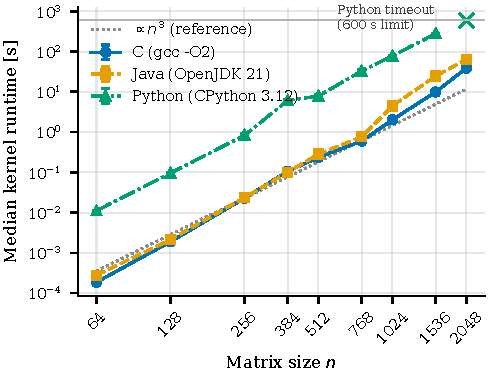
\includegraphics[width=\columnwidth]{runtime_vs_n}
\caption{Median kernel runtime per multiplication vs.\ matrix size (log--log; error bars: IQR, $k=5$ except
Python $n=1536$, $k=3$). Dotted line: $n^3$ reference anchored at the C median for $n=256$. Cross: Python run
stopped by the 600\,s limit at $n=2048$ (no time is reported for it).}
\label{fig:runtime}
\end{figure}

\begin{figure}[t]
\centering
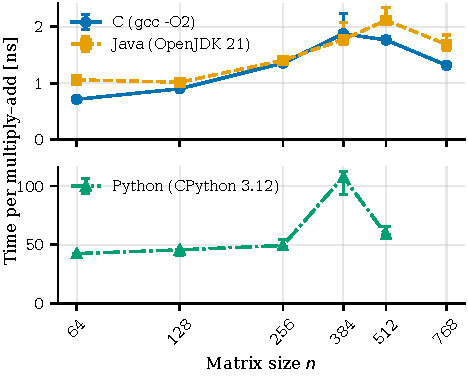
\includegraphics[width=\columnwidth]{ns_per_madd}
\caption{Time per multiply--add, $T/n^3$ (median and IQR of the per-sample values). A flat curve means exact
cubic growth. Python is shown on its own axis because its values are one to two orders of magnitude larger.}
\label{fig:nsmadd}
\end{figure}

\textbf{Time per operation.} \Cref{fig:nsmadd} divides each runtime by the $n^3$ multiply--adds. For C it rises from
\NsMaddCMin{}\,ns at $n=\NsMaddCMinN$ to \NsMaddCTwoFiftySix{}\,ns at $n=256$, stays between about 1.3 and
1.9\,ns up to $n=1024$, and then increases to \NsMaddCFifteenThirtySix{}\,ns ($n=1536$) and
\NsMaddCTwentyFortyEight{}\,ns ($n=2048$). Java stays close to C up to $n=768$ (\NsMaddJavaMin{}--\NsMaddJavaFiveTwelve{}\,ns)
and then rises more steeply: \NsMaddJavaTenTwentyFour{}\,ns at $n=1024$, \NsMaddJavaFifteenThirtySix{}\,ns at
$n=1536$ and \NsMaddJavaTwentyFortyEight{}\,ns at $n=2048$. Python needs \NsMaddPythonMin{}\,ns at $n=64$ and
between \NsMaddPythonTenTwentyFour{} and \NsMaddPythonFifteenThirtySix{}\,ns for $n\ge768$, with an outlier of
\NsMaddPythonThreeEightyFour{}\,ns at $n=384$.

\textbf{Ratios to C at equal $n$} (ratio of medians, 95\,\% bootstrap interval). Java/C is
\RatioJavaSixtyFour{} [\RatioJavaSixtyFourLo, \RatioJavaSixtyFourHi] at $n=64$; between $n=128$ and $n=512$ it lies
between \RatioJavaMin{} and \RatioJavaFiveTwelve{}, and the intervals at $n=128$, 256 and 384 include 1. For larger
$n$ it is \RatioJavaSevenSixtyEight{} [\RatioJavaSevenSixtyEightLo, \RatioJavaSevenSixtyEightHi] at $n=768$,
\RatioJavaTenTwentyFour{} [\RatioJavaTenTwentyFourLo, \RatioJavaTenTwentyFourHi] at $n=1024$,
\RatioJavaFifteenThirtySix{} [\RatioJavaFifteenThirtySixLo, \RatioJavaFifteenThirtySixHi] at $n=1536$ and
\RatioJavaTwentyFortyEight{} [\RatioJavaTwentyFortyEightLo, \RatioJavaTwentyFortyEightHi] at $n=2048$.
Python/C is largest at $n=64$, \RatioPythonSixtyFour{} [\RatioPythonSixtyFourLo, \RatioPythonSixtyFourHi], and falls, not monotonically, to
\RatioPythonTenTwentyFour{} [\RatioPythonTenTwentyFourLo, \RatioPythonTenTwentyFourHi] at $n=1024$ and
\RatioPythonFifteenThirtySix{} [\RatioPythonFifteenThirtySixLo, \RatioPythonFifteenThirtySixHi] at $n=1536$.

\begin{table}[t]
\centering
\caption{Empirical growth exponent $b$ of $T \approx c\,n^b$ (least squares on $\log$ median runtime vs.\ $\log n$) with 95\,\% confidence interval (Student $t$ on the slope). The cubic model predicts $b=3$.}
\label{tab:growth}
\small
\begin{tabular}{@{}llrcc@{}}
\toprule
Implementation & $n$ range & pts & $b$ [95\,\% CI] & $R^2$ \\
\midrule
C & 256--768 & 4 & 2.96 [1.79, 4.14] & 0.9833 \\
C & 64--512 & 5 & 3.49 [3.31, 3.67] & 0.9992 \\
Java & 256--768 & 4 & 3.19 [2.26, 4.13] & 0.9909 \\
Java & 64--512 & 5 & 3.35 [3.10, 3.61] & 0.9983 \\
Python & 256--512 & 3 & 3.35 [-10.93, 17.64] & 0.8991 \\
Python & 64--512 & 5 & 3.29 [2.68, 3.91] & 0.9899 \\
\bottomrule
\end{tabular}
\end{table}


\subsection{Growth exponent}
\Cref{tab:growth} gives the fitted exponents. Over $n=\ExpCNmin$--$\ExpCNmax$, C grows with $b=\ExpC$
[\ExpCLo, \ExpCHi] and Java with $b=\ExpJava$ [\ExpJavaLo, \ExpJavaHi]; neither interval contains 3. Python grows
with $b=\ExpPython$ [\ExpPythonLo, \ExpPythonHi] over $n=\ExpPythonNmin$--$\ExpPythonNmax$, an interval that
contains 3. The restricted fits show the same pattern: for C and Java the exponent is above 3 already for
$n\le512$, and the large-$n$ fits ($n\ge512$) have wide intervals because they rest on only five or four points.

\begin{table}[t]
\centering
\caption{Feasibility limits under the declared budgets (600\,s per process run, 8\,GB memory, $\leq$\,90\,min total benchmark time).}
\label{tab:limits}
\footnotesize
\begin{tabular}{@{}lrrl@{}}
\toprule
Impl. & Largest & Largest & Outcome \\
 & completed $n$ & attempted $n$ & \\
\midrule
C & 2048 & 2048 & none (end of sequence) \\
Java & 2048 & 2048 & none (end of sequence) \\
Python & 1536 & 2048 & timeout at $n=2048$ \\
\bottomrule
\end{tabular}
\end{table}


\subsection{Limits}
C and Java completed every declared size up to $n=2048$ (\cref{tab:limits}). The single Python attempt at
$n=\PyFailN$ was stopped by the \PyFailWall\,s limit (status \texttt{\PyFailType}); it is recorded without a time.
The largest feasible Python size under the declared budget is therefore $n=\MaxNPython$. No configuration came
close to the 8\,GB memory budget.

\begin{table}[t]
\centering
\caption{Memory at the largest completed $n$ of each implementation. Peak RSS: median over the measured process runs (GNU \texttt{time} \%M); baseline: median peak RSS of the same program at $n=1$ ($k=5$). Language metric: C \texttt{matrix\_storage\_bytes} (exact allocation), Java \texttt{jvm\_heap\_peak\_used\_bytes} (MemoryPoolMXBean, heap pools), Python \texttt{pyobj\_deep\_size\_bytes} (\texttt{sys.getsizeof}). The metrics measure different things and are not directly comparable.}
\label{tab:memory}
\footnotesize
\setlength{\tabcolsep}{2.5pt}
\begin{tabular}{@{}lrrrrrr@{}}
\toprule
Impl. & $n$ & RSS & Baseline & RSS$-$base & $3\cdot8n^2$ & Lang. metric (B/elem.) \\
 & & [MiB] & [MiB] & [MiB] & [MiB] & [MiB] \\
\midrule
C & 1536 & 55.8 & 1.9 & 54.0 & 54.0 & 54.0 (8.0) \\
C & 2048 & 97.9 & 1.9 & 96.0 & 96.0 & 96.0 (8.0) \\
Java & 1536 & 142.4 & 48.2 & 94.2 & 54.0 & 96.9 (14.4) \\
Java & 2048 & 184.7 & 48.2 & 136.5 & 96.0 & 138.4 (11.5) \\
Python & 1536 & 283.4 & 12.5 & 270.9 & 54.0 & 216.3 (32.0) \\
\bottomrule
\end{tabular}
\end{table}


\begin{figure}[t]
\centering
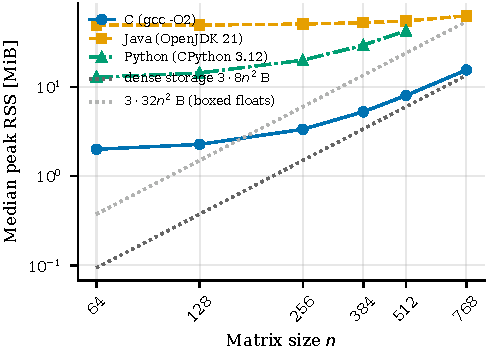
\includegraphics[width=\columnwidth]{memory_rss}
\caption{Median peak RSS of the whole process (GNU \texttt{time}) vs.\ matrix size. Dotted lines: storage of the
three matrices at 8\,B per element (dense) and at 32\,B per element (Python estimate: 24\,B \texttt{float} object +
8\,B list reference).}
\label{fig:memory}
\end{figure}

\subsection{Memory}
The runtime alone, measured at $n=1$, occupies \RssBaseC{}\,MiB (C), \RssBaseJava{}\,MiB (Java) and
\RssBasePython{}\,MiB (Python) of peak RSS. For small $n$ this baseline dominates (\cref{fig:memory}): Java stays
near 50\,MiB up to $n=512$. At the largest common size $n=\MemCommonN$ the peak RSS is \RssCommonC{}\,MiB (C),
\RssCommonJava{}\,MiB (Java) and \RssCommonPython{}\,MiB (Python); after subtracting the baseline this is
\RssNetCommonC{}, \RssNetCommonJava{} and \RssNetCommonPython{}\,MiB, compared with \DenseCommon{}\,MiB for three
dense float64 matrices (\cref{tab:memory}). The language-specific metrics give \MemMetricBpeC{}\,B per element for
C (exact allocation), \MemMetricBpeJava{}\,B per element for the Java heap peak at $n=2048$ and
\MemMetricBpePython{}\,B per element for the Python object graph.

\begin{figure}[t]
\centering
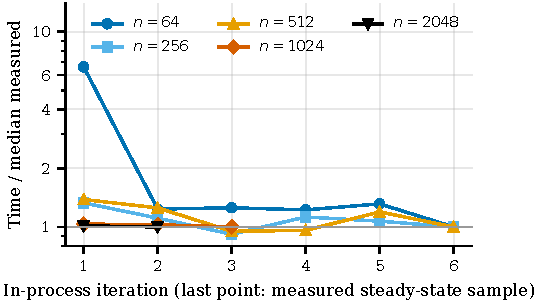
\includegraphics[width=\columnwidth]{java_warmup}
\caption{Java JIT warm-up: time of each in-process warm-up iteration divided by the median of the measured
samples at the same $n$ (median over the $P=5$ processes; log scale). The last point is the measured sample.}
\label{fig:warmup}
\end{figure}

\subsection{Warm-up and variability}
In Java the first in-process iteration takes \JavaFirstIterMaxRel{} times the steady-state median at
$n=\JavaFirstIterMaxRelN$, while at $n=\JavaFirstIterLargeN$ it takes \JavaFirstIterLargeRel{} times
(\cref{fig:warmup}). In C and Python the first iteration is between \CFirstIterRelMin{}--\CFirstIterRelMax{} and
\PythonFirstIterRelMin{}--\PythonFirstIterRelMax{} times the median, respectively, i.e.\ there is no systematic
warm-up effect. The relative IQR (IQR/median) has a median over the sizes of \RelIQRCMedian\,\% (C),
\RelIQRJavaMedian\,\% (Java) and \RelIQRPythonMedian\,\% (Python); its maximum occurs at $n=384$ for all three
languages (\RelIQRCMax\,\%, \RelIQRJavaMax\,\% and \RelIQRPythonMax\,\%), a size measured in session~1, when the
machine was busy (load average up to \SessionOneLoadMax{} in that session). Two configurations mix sessions: Python at $n=768$ (session~1 median
\MixedPythonSevenSixtyEightSessionOneMedian{}, $k=\MixedPythonSevenSixtyEightSessionOneK$; session~2
\MixedPythonSevenSixtyEightSessionTwoMedian{}, $k=\MixedPythonSevenSixtyEightSessionTwoK$) and Python at
$n=1536$ (session~2 \MixedPythonFifteenThirtySixSessionTwoMedian{}, $k=\MixedPythonFifteenThirtySixSessionTwoK$;
session~3 \MixedPythonFifteenThirtySixSessionThreeMedian{}, $k=\MixedPythonFifteenThirtySixSessionThreeK$).

\begin{table}[t]
\centering
\caption{Separate experiment (not part of the language comparison): same C source compiled with different gcc flags. Median [IQR] kernel runtime, $k=5$ process runs, 1 warm-up each.}
\label{tab:cflags}
\scriptsize
\setlength{\tabcolsep}{3pt}
\begin{tabular}{@{}lrrr@{}}
\toprule
gcc flags & $n=256$ & $n=512$ & $n=1024$ \\
\midrule
\texttt{-O0} & 59.9\,ms [2.27\,ms] & 495\,ms [13\,ms] & 4.32\,s [49\,ms] \\
\texttt{-O2} & 20.8\,ms [1.64\,ms] & 180\,ms [1.77\,ms] & 1.57\,s [11\,ms] \\
\texttt{-O3} & 22.2\,ms [268\,\textmu s] & 176\,ms [675\,\textmu s] & 1.5\,s [11.7\,ms] \\
\texttt{-O3 -march=native} & 20.5\,ms [1.79\,ms] & 176\,ms [4.5\,ms] & 1.51\,s [23.8\,ms] \\
\bottomrule
\end{tabular}
\end{table}


\subsection{Separate experiment: C compiler flags}
At $n=\CflagsN$ (\cref{tab:cflags}), \texttt{-O0} is \CflagsOzeroOverOtwo{} times slower than \texttt{-O2}, while
\texttt{-O3} and \texttt{-O3 -march=native} take \CflagsOthreeOverOtwo{} and \CflagsNativeOverOtwo{} times the
\texttt{-O2} median. The checksums of the four variants are identical at every $n$. The \texttt{-O2} median of this
experiment at $n=1024$ (\CflagsOtwoMedian{}, session~3) is lower than the \TCTenTwentyFour{} measured for the same
binary in the size sweep (session~2).

% ------------------------------------------------------------------ Discussion
\section{Discussion}
\label{sec:discussion}

\subsection{Answer to the research question}
On the tested laptop, all three implementations perform exactly $n^3$ multiply--adds, but only the Python runtime
grows at a rate compatible with $n^3$ ($b=\ExpPython$). The C and Java runtimes grow faster ($b=\ExpC$ and
$b=\ExpJava$) because the time per multiply--add increases with $n$. At equal $n$, C and Java cannot be told apart
for $128\le n\le384$; from $n=768$ on, Java is slower by a factor between \RatioJavaSevenSixtyEight{} and
\RatioJavaFifteenThirtySix{}. Python is \RatioPythonMin{}--\RatioPythonMax{} times slower than C and is the only
implementation that does not finish $n=2048$ within 600\,s. In memory, the fixed runtime cost dominates for small
$n$ (Java about \RssBaseJava{}\,MiB), while for large $n$ C uses exactly the dense storage and Python about five
times as much.

\subsection{Hypotheses}
\emph{H1 (cubic growth) is partially supported.} The operation count is cubic by construction and the Python
exponent interval contains 3, but the C and Java intervals exclude 3 over the main range and for $n\le512$ (the
fits for $n\ge512$ have only five points and are too wide to decide for C). The predicted
deviation at large $n$ is present, and for C and Java it already appears at small $n$.
\emph{H2 (C $<$ Java $<$ Python, Java within a small factor) is supported with a qualification.} Python is always
the slowest, and Java is at most \RatioJavaMax{} times slower than C. However, C is not measurably faster than Java
at $n=128$--384, so the order C $<$ Java holds only where the bootstrap intervals exclude 1 ($n=64$ and $n\ge512$).
\emph{H3 (more memory per element in Python) is supported.} \texttt{sys.getsizeof} gives \MemMetricBpePython{}\,B
per element against 8\,B in C, and the peak RSS above the baseline at $n=\MemCommonN$ is \RssNetCommonPython{}\,MiB
against \RssNetCommonC{}\,MiB.

\subsection{Interpretation}
\textbf{Memory hierarchy (C).} The steps in the C time per multiply--add line up with the size of $B$ ($8n^2$\,B)
relative to the caches of \cref{tab:env}. $B$ fills the 32\,KiB L1d at $n=64$ (\NsMaddCSixtyFour\,ns), fits in the
256\,KiB L2 at $n=128$ (\NsMaddCOneTwoEight\,ns), and needs the 12\,MiB L3 at $n=256$--1024 (8\,MiB at $n=1024$).
It exceeds L3 at $n=1536$ (18\,MiB, \NsMaddCFifteenThirtySix\,ns) and $n=2048$ (32\,MiB, \NsMaddCTwentyFortyEight\,ns).
In the ijk order every access to $B$ jumps $8n$ bytes, so each one uses a new cache line and, for $n\ge512$, a new
4\,KiB page. This is the access pattern that Drepper uses to show the cost of cache and TLB misses~\cite{drepper2007}.
The power-of-two sizes may add cache-set conflicts~\cite{lam1991}, which this design cannot separate from capacity
effects. Hardware counters were not available (\texttt{perf\_event\_paranoid}$=4$), so these explanations agree
with the data but are \emph{not verified} here.

\textbf{Java layout and JIT.} After warm-up, Java matches C while the working set is cache-resident, which
indicates that the JIT-compiled loop is about as fast as the gcc~\texttt{-O2} loop when memory is not the
bottleneck. The gap opens exactly when C also slows down (from $n=768$--1024), so Java appears to be more sensitive
to the memory hierarchy. A plausible but unverified cause is the \texttt{double[][]} layout. Every access
\texttt{b[k][j]} first loads the reference to row $k$, and the rows are separate heap objects with headers and no
guaranteed contiguity or alignment. Confirming this would require cache-miss counters or the JIT-generated
assembly. The JIT effect itself is clear in \cref{fig:warmup}. The first iteration is much slower only for short
kernels, which run mostly in the interpreter or in early compilation tiers~\cite{georges2007}. At $n\ge1024$ the
first iteration already takes about as long as the steady state, so JIT compilation happens within its first small
fraction.

\textbf{Interpreter cost (Python).} CPython runs every multiply--add as several bytecode instructions with list
indexing and creates a new \texttt{float} object for each product and partial sum~\cite{pep659,pydocsys}. This
fixed cost per operation, \NsMaddPythonMin--\NsMaddPythonFifteenThirtySix\,ns compared with \NsMaddCMin--\NsMaddCMax\,ns in C,
explains three observations. The exponent is close to 3, the ratio to C is large, and the ratio falls as $n$ grows,
because C becomes memory-bound while Python remains interpreter-bound. The moderate increase of the Python time per
operation with $n$ may also be a memory effect: the process reaches \RssPythonFifteenThirtySix\,MiB of peak RSS at
$n=1536$. This is a conjecture. The outlier at $n=384$ was measured in the busiest session and is treated as
measurement variability, not as a property of the algorithm.

\textbf{Memory.} For C the peak RSS above the baseline equals the dense storage ($\RssOverDenseC\times$ at
$n=\RssMaxNnC$), as expected from three \texttt{malloc}ed blocks. The 32\,B per element measured for Python matches
a 24\,B \texttt{float} object plus an 8\,B list reference. The peak RSS is somewhat higher still
($\RssOverDensePython\times$ the dense storage, i.e.\ more than $4\times$). The remaining difference
(allocator overhead and temporary buffers created while loading the inputs) is not attributed here. Java needs
$\RssOverDenseJava\times$ the dense storage above its baseline at $n=\RssMaxNnJava$. The JVM heap metric also
includes objects that were not yet collected, so it is an upper bound of the live matrix data rather than an exact
size.

\textbf{Compiler flags.} Turning optimisation off costs a factor \CflagsOzeroOverOtwo{}, whereas \texttt{-O3} and
\texttt{-march=native} change the time by less than 10\,\% at every tested $n$. A plausible explanation is the reduction
\texttt{s += a*b}. GCC does not reassociate floating-point operations by default (\texttt{-fno-associative-math}),
and no \texttt{-O} level below \texttt{-Ofast} enables this~\cite{gccopt}. The compiler therefore has to keep the
sequential order of the sum, which prevents the usual SIMD reduction. The identical checksums of all variants are
consistent with an unchanged evaluation order.

\subsection{Limitations}
(i)~One laptop with the \texttt{powersave} governor and turbo enabled. The clock frequency depends on temperature
and on the number of active cores, and the three sessions ran under different loads. The same \texttt{-O2} binary
gave \TCTenTwentyFour{} at $n=1024$ in session~2 and \CflagsOtwoMedian{} in session~3, so the difference between
sessions can exceed the IQR within a session. Comparisons between sizes measured in different sessions should
therefore be read with this uncertainty in mind.
(ii)~Other agents shared the machine. The lock serialised all timed runs, but not other work such as compilation.
(iii)~No hardware counters, so the explanations based on caches and memory layout remain conjectures.
(iv)~Few samples where runs are expensive: $k=3$ for Python at $n=1536$ and a single attempt at $n=2048$.
Bootstrap intervals from $k=5$ are approximate.
(v)~Each language uses its idiomatic layout. The results therefore compare implementations as written, not the
languages in general. The language-specific memory metrics are not comparable with one another; only the peak RSS
is.
(vi)~One input distribution (uniform $[-1,1)$) and square matrices only.

% ------------------------------------------------------------------ Conclusions
\section{Conclusions}
\label{sec:conclusions}
For the naive ijk float64 multiplication on an Intel Core i7-9750H laptop, with gcc~13.3 \texttt{-O2}, OpenJDK~21
and CPython~3.12, the study establishes the following points.
(1)~The three implementations are correct and bit-identical, so the comparison measures only how fast each one
executes the same arithmetic.
(2)~The runtime grows faster than the cubic operation count for C and Java ($b\approx\ExpC$ and $\ExpJava$),
because the cost per multiply--add rises from \NsMaddCMin{} to \NsMaddCMax\,ns in C. For Python it grows roughly as
$n^3$, because the interpreter cost per operation dominates.
(3)~Java is as fast as C for cache-resident sizes and up to \RatioJavaMax{} times slower for larger ones. Python is
\RatioPythonMin--\RatioPythonMax{} times slower than C, and its largest feasible size under a 600\,s budget is
$n=\MaxNPython$.
(4)~The memory per element is 8\,B in C and 32\,B in Python, and the runtime baseline dominates the peak RSS of
Java and Python at small $n$.
These statements hold only for the tested implementations, settings, inputs and hardware. Several questions remain
open. Hardware counters are needed to confirm the cache, TLB and layout explanations, including the specific cause
of the Java gap. A contiguous one-dimensional Java array would show how much of the gap the layout explains.
Measuring all sizes in one session would remove the variability between sessions. Loop reordering, blocking and
parallel execution are left to the following assignments.

% ------------------------------------------------------------------ Materials + AI statement
\section*{Reproducibility Materials}
Repository: \url{https://github.com/danirodriguezz/bigdata-assignment01-matmul-languages} (submitted version: tag
\texttt{v1.0-submission}); the same content is in \texttt{Assignment01\_RodriguezAlonso\_Materials.zip}. It
contains the source code (\texttt{src/}), the correctness tests (\texttt{tests/}), the input generator and
experiment driver (\texttt{scripts/}), the configuration (\texttt{configs/experiment.json}), all raw measurements
(\texttt{results/raw/*.csv}, schema in \texttt{results/README.md}), the environment snapshot, the analysis scripts
that produce every table, figure and number of this report (\texttt{analysis/make\_all.py}) and this report's
source. \texttt{make setup test inputs bench analysis report} reproduces the study; \texttt{make analysis report}
regenerates all tables and figures from the committed raw data.

\section*{Use of Generative AI}
Claude Code (Anthropic), model Claude Opus 5.5, was used as an assistant to plan the experiment, to draft and
debug the C, Java and Python programs, the correctness tests, the benchmark driver and the analysis scripts, to
draft the text of this report and the README, and for language revision. All measurements were produced by runs on
the author's laptop and are stored in the repository; no result was generated or estimated by the tool. Every
reference was checked against its DOI or publisher record or its official URL. The author reviewed the code, the
data and the text and is responsible for the content.

% ------------------------------------------------------------------ References
\bibliographystyle{IEEEtran}
\bibliography{references}

\end{document}
